\section{High-Level Objective}
\subsection{Product}
Suttung tasked the authors to implement a new game object model for the NOX Engine, named NOX ECS.
NOX ECS would be an alternative to the existing NOX Actor system.
The new component systems would look into different methodologies for organizing its data, and also
be able to take advantage of multi-core CPUs.
The NOX ECS would be based on requirements agreed upon by Suttung and the authors.

\begin{figure}[H]
    \begin{center}
    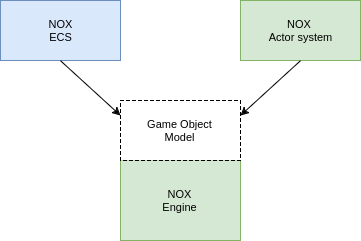
\includegraphics[scale=0.45]{images/ecs_vs_actor_distinction.png}
    \caption[NOX ECS versus NOX Actor]{The figure shows how the NOX ECS fits into the NOX Engine picture. The figures colored in green was developed by Suttung, the figure in blue is our NOX ECS}
    \label{fig:ecs_vs_actor_distinction}
    \end{center}
\end{figure}

\subsection{Research}
In addition to this task given by Suttung, we also decided that we could use this task to discuss
multi-threaded entity component systems at a more general level, making it more relevant for a broader audience.
We decided to discuss the implementation of the NOX ECS compared to the more object oriented NOX Actor system,
and discuss the findings in a more general setting.
